%Plan de tests
%Recette du commanditaire 
\subsection{Qualité d'extraction de texte}\label{testOCR}
%tests de l'OCR sur un échantillon de documents
Le module d'extraction de texte par OCR est critique, car sa sortie détermine ensuite la qualité de l'indexage et de la classification du document.
Si le module retourne un texte incorrect, avec des fautes et/ou des lettres modifiées, les modules d'extraction de métadonnées ou de taxonomies ne pourront pas reconnaitre correctement les mots clefs.
Cela est d'autant plus vrai que nos méthodes de détection par RegEx sont par nature très sensibles au format du texte a détecter.


La qualité d'extraction de l'\gls{ocr} est directement corrélée au prétraitement d'image.
Nous voulions obtenir les meilleurs paramètres pour ce prétraitement afin d'obtenir une qualité d'extraction optimale pour notre cas d'application.
Nous avons effectué plus de 50 tests avec différents paramètres de traitement graphique.

Deux métriques de test ont été utilisées pour évaluer les performances de notre OCR\@.

La première méthodes se base sur la distance par rapport au texte de base.
Cette méthode nécessitait un ensemble de documents dont les transcripts étaient connus, et la première étape fut de transcrire à la main les seuls 12 documents administratifs que nous avions au début du projet.

La deuxième méthode est de compter les informations d'importances présentes dans le sortie de l'OCR par rapport a une liste de référence.
Nous avons sélectionné une liste de mots clefs que nous estimions importants, comme des noms ou des dates, et relevé leurs présences dans chaque documents dans un fichier a part.

Il faut se replacer dans le contexte du début de projet: a cette époque nous n'avions encore que quelques documents exemple, et nous n'avions pas défini les informations importantes avec le commanditaire.
De plus nous n'avions pas encore réduit le cadre du projet pour ne traiter que les RAA donc la diversité des documents était plus grande.



La première métrique d'évaluation de qualité de texte est celle des mots clefs.

On calcule le pourcentage de mots clefs extraits correctement en comptant simplement le nombre de mots clefs présents dans le texte en sortie de l'OCR divisé par le nombre de mots clefs total trouvé précédent. 


La deuxième métrique est la distance de Levenshtein.

Cette distance indique le degré de séparation entre deux chaines de caractères, c'est a dire le nombre minimum de modifications (ajout, suppression, modifications) a faire pour passer d'une chaine a l'autre. Elle est donnée par la formule suivante:

\begin{equation}
	\text{lev}_{a,b}(i,j) = \left\{\begin{matrix}
		\text{max}(i,j) & \text{si min}(i,j) = 0 \\ 
		\text{min}\left\{\begin{matrix}
			\text{lev}_{a,b}(i-1,j)\\ 
			\text{lev}_{a,b}(i,j-1)\\ 
			\text{lev}_{a,b}(i-1,j-1)+1_{a_i \neq b_j}
		\end{matrix}\right. & \text{sinon} \\ 
	\end{matrix}\right.
\end{equation}

Pour chaque document, nous obtenons donc 2 valeurs de métriques nous donnant une indication sur la qualité du texte extrait.

Pour trouver les meilleurs paramètres du prétraitement, nous devions donc trouver la méthode qui donnerait le meilleur score pour les deux métriques.
Nous avons donc procédé a une analyse statistique, en testant plus d'une cinquantaine de paramètres de traitement graphique différents.

Pour chacun de ces paramètres nous avons calculé la distance de Levenshtein ainsi que le pourcentage de mots clefs correctement extraits.
Nous avons ensuite calculé la variance ainsi que la moyenne pour chacune de ces deux métriques.
L'ensemble des paramètres sont alors normalisés, c'est a dire que la méthode de traitement qui donne les meilleurs résultats obtient un score de 100, et la pire méthode obtient un score de 0.
Après élimination des cas extrêmes qui provoquent l'aplatissement des valeurs `normales', nous avons été en mesure de choisir les paramètres qui nous semblaient donner la meilleure combinaison de résultats.


\begin{figure}[h!]
  \centering
  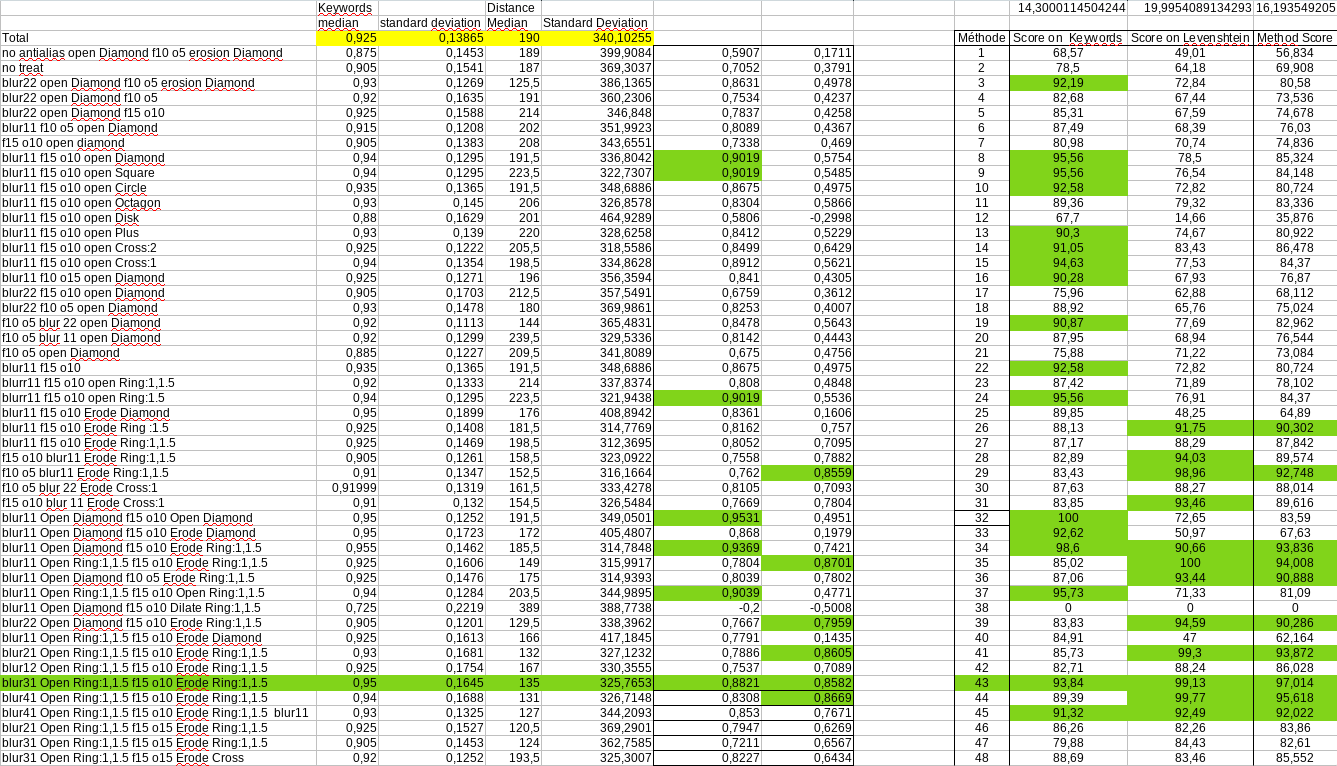
\includegraphics[width=0.7\textwidth]{ocrAnalysis.png}
	\caption[]{Résultat des tests de traitement d'image et les scores associés (meilleur résultat en vert)}
	\label{fig:ocrRes}
\end{figure}

La colonne la plus a droite `Method score' est une simple formule mathématique qui détermine le score de la méthode étudiée.
Cette formule favorise le score de la distance de Levenshtein, dont les variations sont bien plus significatives que les variations du score des mots clef pour la qualité d'un document.

%Pour comparer toutes les métriques, on a normalisé entre tout les documents (100 pour la meilleure méthodes et 0 pour la pire, avec elimination des outliers)
%Deux méthodes: transcripts et mots clefs

\subsection{Test des métadonnées}
Comme mentionné précédemment dans la partie réalisation, nous avons mené une étude poussée des documents pour relever toutes les variations de notation de chaque informations d'importance.
Ces résultats nous ont permis d'obtenir une liste exhaustive des formats de données.
Les RegEx ont été écrits sur un \href{https://regex101.com/}{site internet} de test en ligne sur l'ensemble des formats trouvés précédemment (exemple sur la figure~\ref{fig:regexRAA}).

Si l'ensemble des exemples est pris en compte et que les contres exemples sont exclus, nous considérons alors que le RegEx est valide.

Nous testons ensuite la detection sur plusieurs documents en relevant les résultats incorrects et corrigeant les RegEx en fonction.


\subsection{Taxonomie}
Comme nous ne possédions pas de corpus de données annoté, et que nous ne sommes pas des experts dans la classification de documents administratifs, le développement d'une procédure de test était hors de notre portée.
C'est un travail spécialisé qui demande une expertise que nous n'avons pas.

Néanmoins, quelques méthodes nous ont permis de mieux juger de la qualité de la taxonomie extraite par ce module. 

Nous avons utilisé un script de test, qui passait au module taxonomique des chaines de caractères contenant des termes taxonomiques se trouvant dans le fichier taxonomique.
En comparant simplement les résultats, on pouvait vérifier que notre programme renvoyait effectivement les termes taxonomiques correspondants.
Avec cette méthode, nous étions capable de vérifier si les modifications dans le module taxonomique provoquait des dysfonctionnements au niveau de sa sortie. 

Ensuite, nous avons passé au module taxonomique des titres provenant de documents administratifs réels, dont nous connaissons les classements taxonomiques évidents.
Ainsi, nous avons pu découvrir et corriger plusieurs bugs, car nous savions exactement a quoi nous attendre.

Pour tenter de détecter et de corriger le plus d'erreurs possible nous avons essayé le module taxonomique avec une très grande quantité de documents, vérifiant a chaque fois à la main la sortie de celui ci. 

C'est cependant lorsque le module `moteur de recherche' fut implémenté que nous avons pu vraiment voir les bugs les moins évidents.
L'affichage du moteur de recherche permet de voir une liste exhaustive des taxonomies, et certaines taxonomies n'étaient pas présentes.
Ce bug était du a un problème du parcours de l'arbre taxonomique.


Notre version finale revoit une taxonomie correcte, validée avec le commanditaire.

%test de la recherche taxonomique
%"outre mer" "delegation de signature"


%Test des métadonnées

